
\definecolor{lightRed}{RGB}{255,115,115}

%%%%%%%%%%

\begin{frame}{\vskip -0.2cm \large L'algorithme CART de Breiman-Friedman-Olshen-Stone}

\small

\begin{multicols}{2}

	\begin{flushright}
	\begin{minipage}{4.5cm}
	\vskip -0.4cm
	{\color{white}AAA}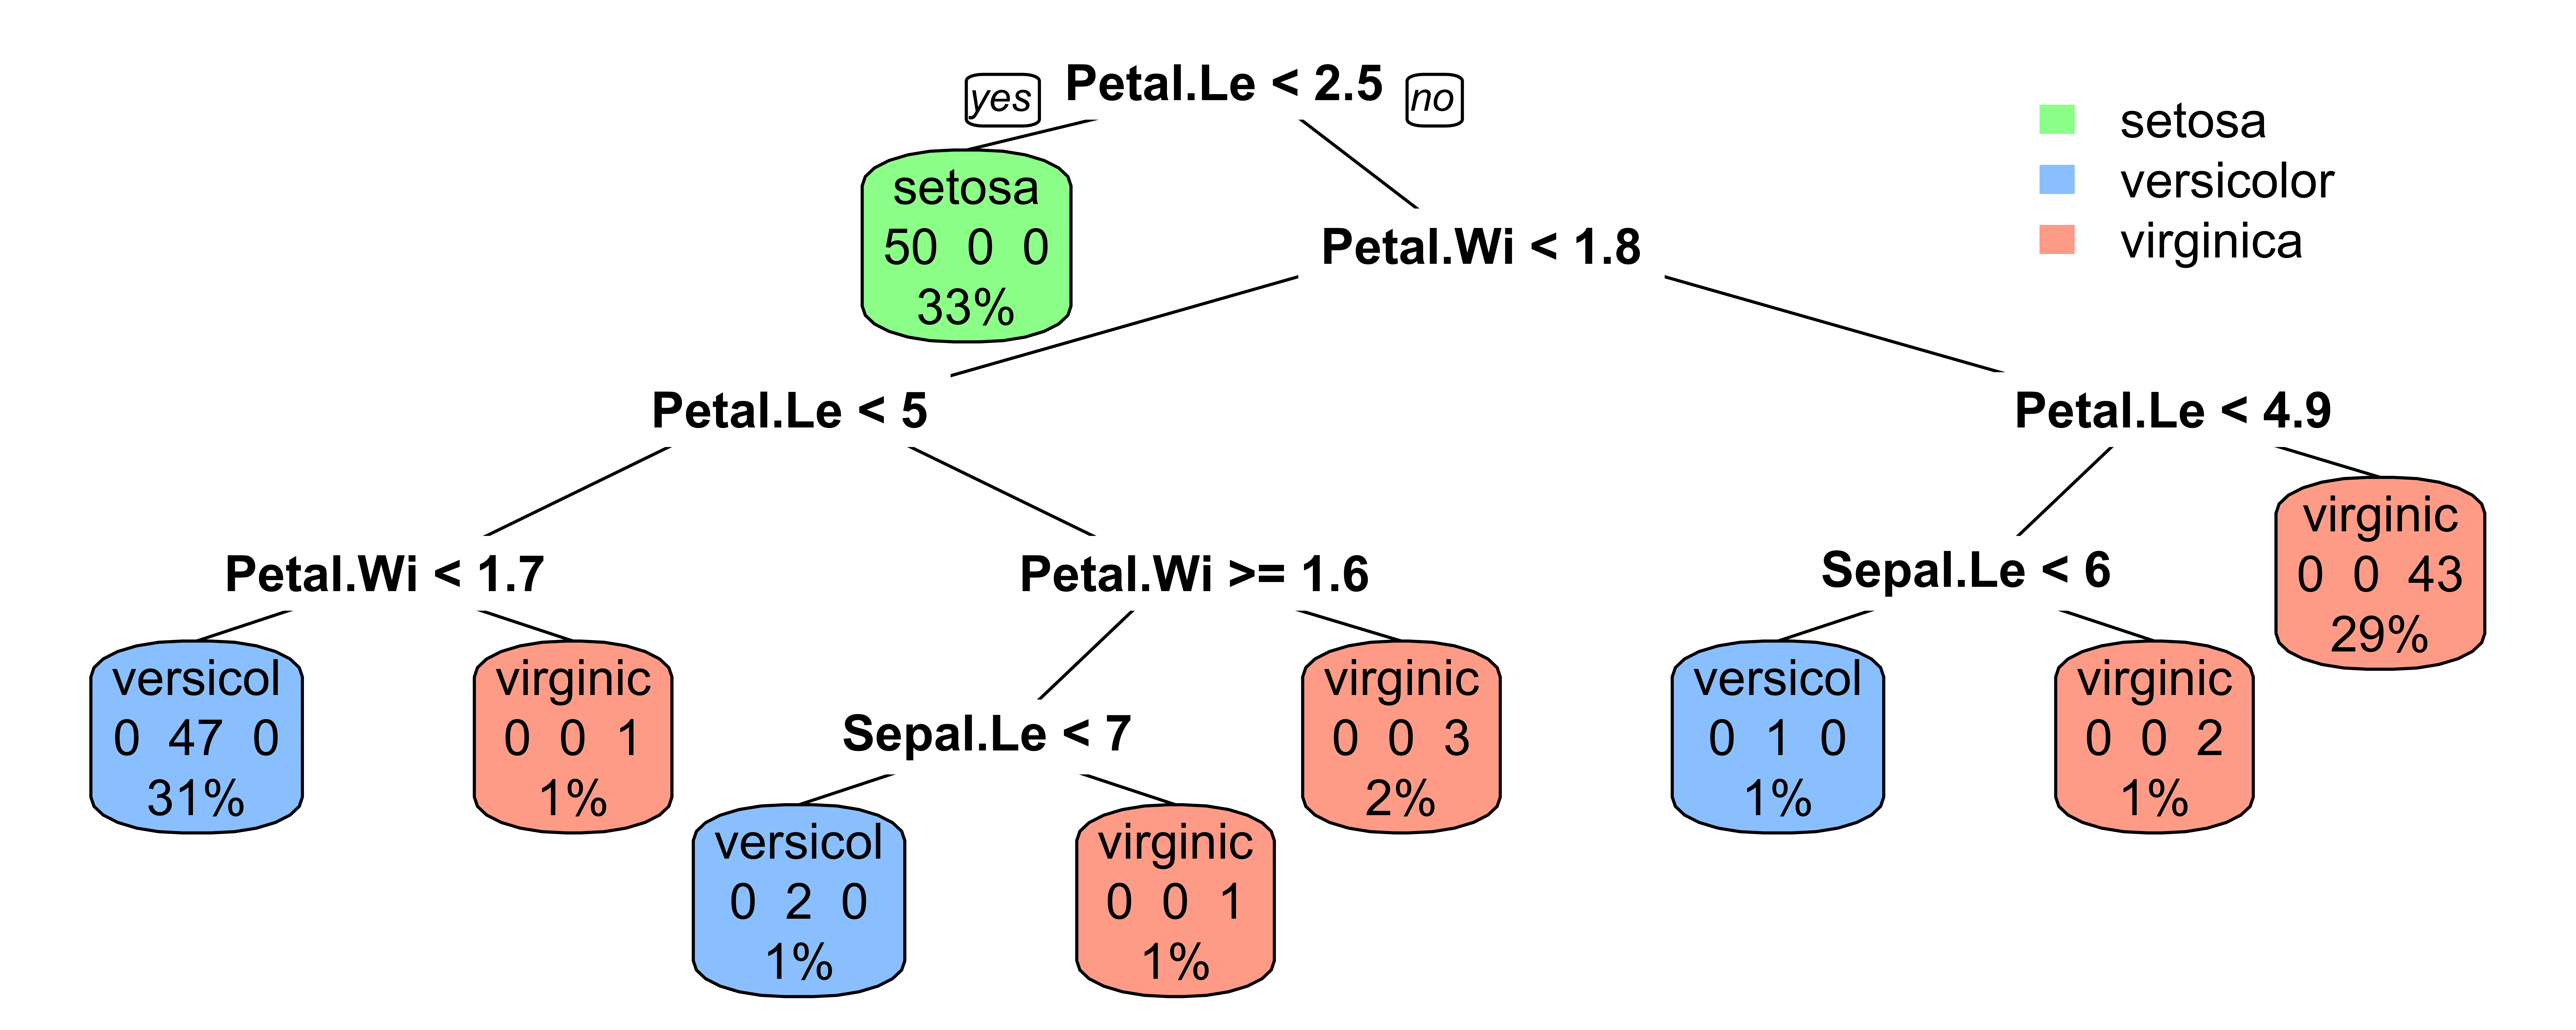
\includegraphics[height=3.5cm]{graphics/plot-rpart.png}
	\vskip 0.1cm 
	{\color{white}AA}
	\includegraphics[height=3.5cm]{graphics/scatter-petalLength-vs-petalWidth-boundaries.png}
	%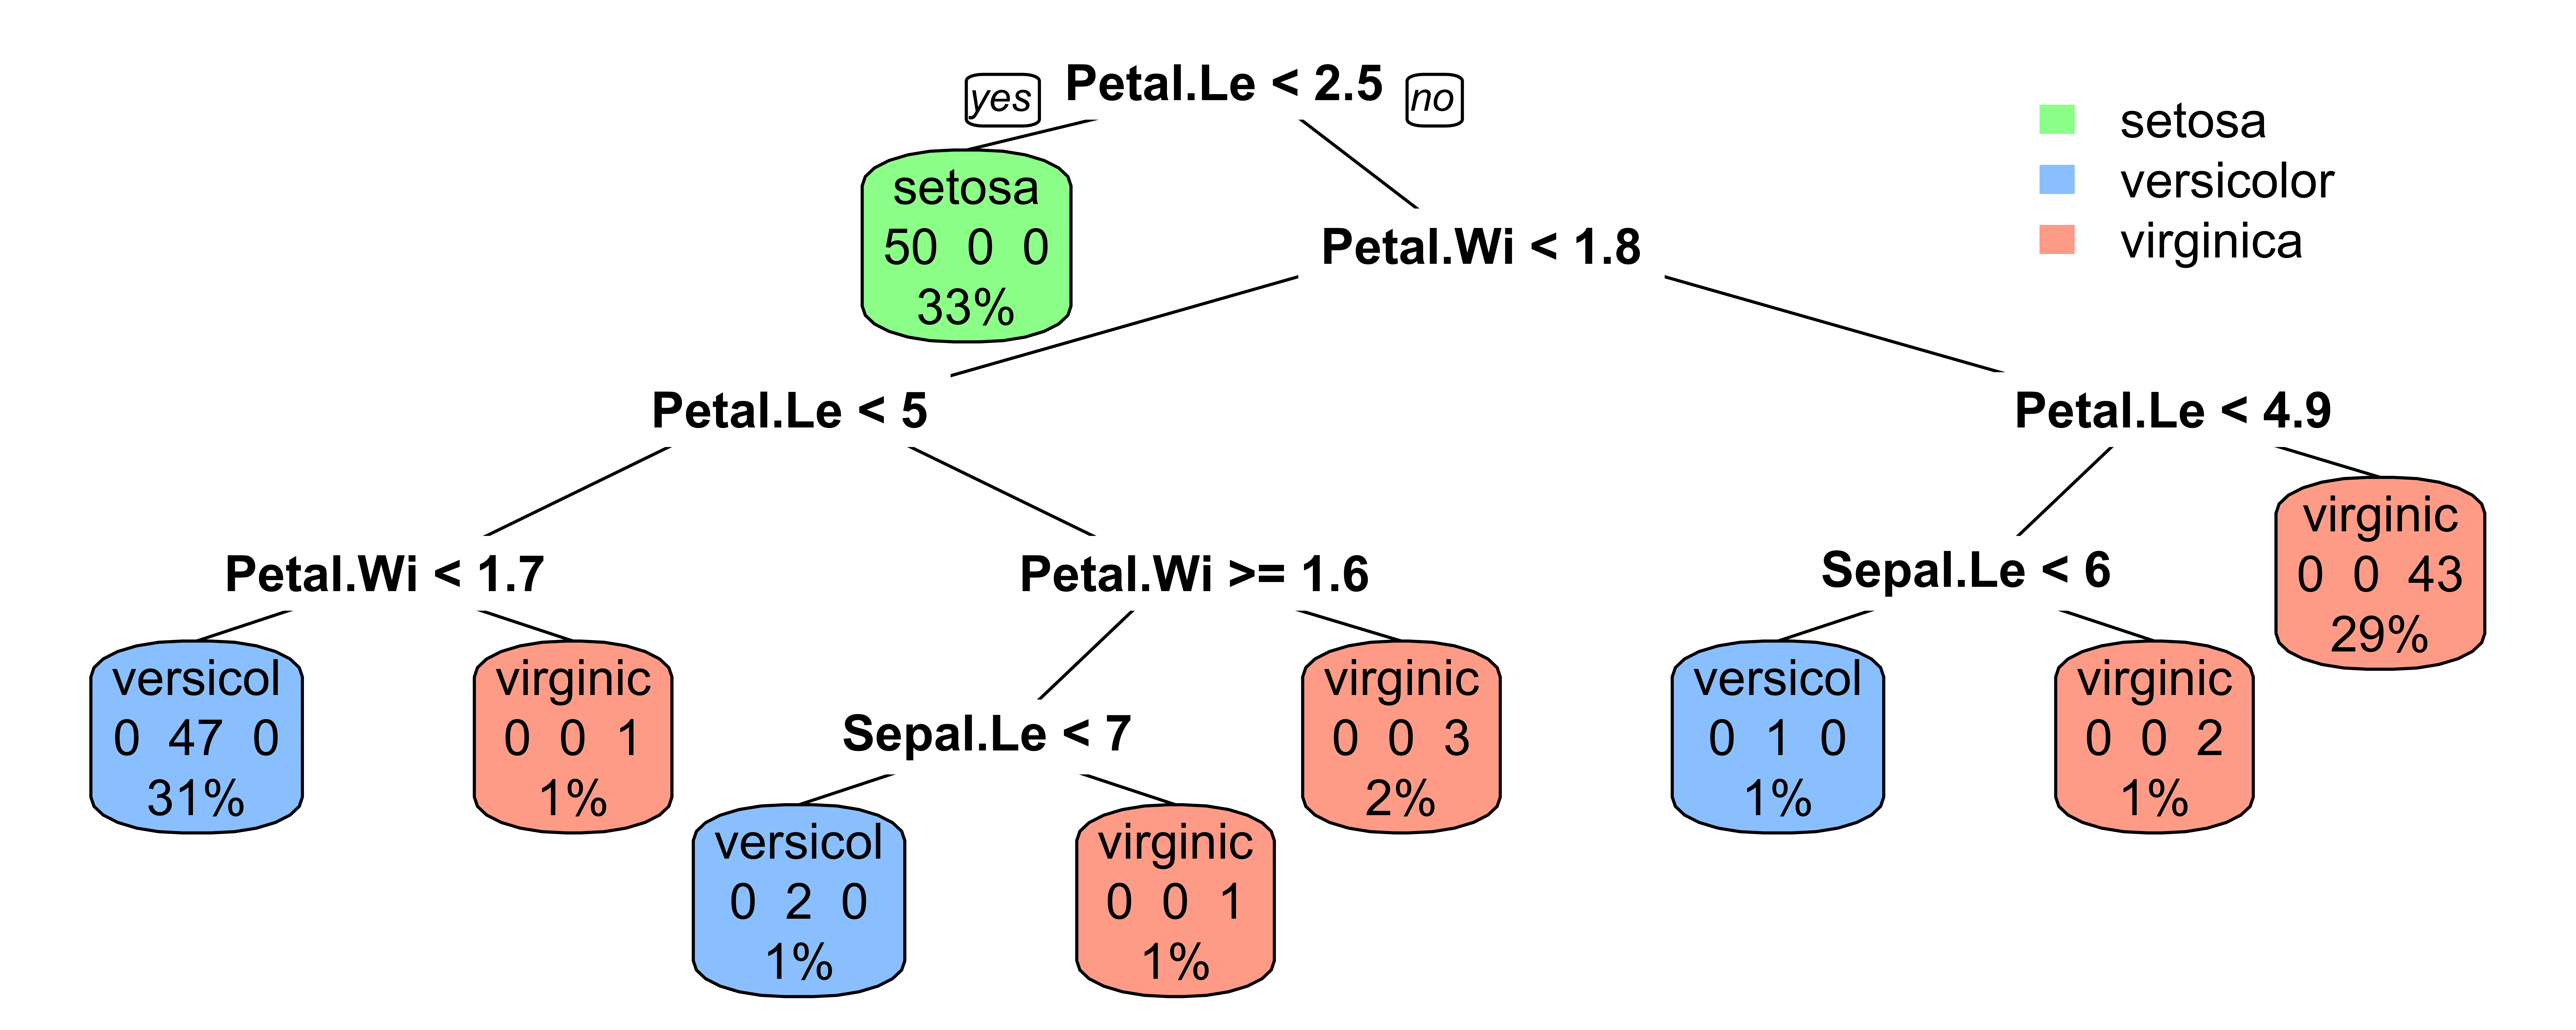
\includegraphics[width=4.5cm,height=6.25cm]{graphics/plot-rpart.png}
	%\includegraphics[width=4.5cm]{graphics/scatter-petalLength-vs-petalWidth-boundaries.png}
	\end{minipage}
	\end{flushright}

\columnbreak

	\begin{flushleft}
	\begin{minipage}{5.75cm}
	\vskip -0.5cm
	%{\tiny
	%\begin{itemize}
	%\item
	%	\pause
	%	But: trouver l'arbre qui minimise l'impuret\'e.
	%\item
	%	\pause
	%	Classe d'hypoth\`eses est essentiellement finie (given data),
	%	mais normalement trop \'enorme;
	%	\pause
	%	recherche exhaustive ne marchera pas.
	%\end{itemize}}
	\scriptsize
	\pause
	\textbf{\normalsize L'algorithme CART} {\tiny(\'etape de croissance)}
	\begin{itemize}
	\item
		\pause
		\`A chaque it\'eration, partitionner \textbf{\color{red}chaque} feuille en deux pour obtenir l'arbre prochain
	\item
		\pause
		Pour chaque feuille, il faut donc choisir:
		\vskip -0.15cm
		\begin{itemize}
		\setlength{\itemindent}{-0.15in}
		\item
			\pause
			{\scriptsize
			\vskip -0.1cm la \guillemotleft\;meilleure \guillemotright\;variable pr\'edictive par
			\vskip -0.1cm {\color{white}.}\!\!\!\!\!\!\!\!\!\!\! laquelle \`a partitionner
			}
		\item
			\pause
			\vskip -0.1cm {\scriptsize le \guillemotleft\;meilleur \guillemotright\;seuil}
		\end{itemize}
	\item
		\pause
		In\'egalit\'e de Jensen \,$\Longrightarrow$\,
		{\color{red}l'impuret\'e d'arbre d\'ecro\^it toujours apr\`es le partitionnement d'une feuille.}
	\item
		\pause
		Pour chaque feuille, choisir la (variable,{\color{white}.}seuil)-combo
		qui maximise la d\'ecroissance d'impuret\'e.
	\item
		\pause
		Pour chaque feuille, continuer jusqu'\`a ce que le crit\`ere d'arr\^et soit satisfait.
	%\item
	%	\pause
	%	Complexit\'e algorithmique = $O\!\left(p\,n \log n\right)$
	\end{itemize}
	\end{minipage}
	\end{flushleft}

\end{multicols}

\end{frame}
\normalsize

%%%%%%%%%%

\begin{frame}{\vskip -0.2cm \large L'algorithme CART de Breiman-Friedman-Olshen-Stone}

\Large
\textbf{L'algorithme CART } {(\'etape d'\'elagage)}

\vskip 0.1cm
\scriptsize
\begin{itemize}
\pause
\item
	Pour plus de d\'etails, voir:
	\vskip -0.2cm
	{\tiny\begin{itemize}
	\item
		{\tiny Breiman-Friedman-Olshen-Stone, (1984),
		\textit{Classification and Regression Trees}, Taylor \& Francis}
	\item
		\vskip -0.1cm
		{\tiny Ripley, (1996),
		\textit{Pattern Recognition and Neural Networks}, Cambridge University Press}
	\end{itemize}}
\pause
\item
	%The tree-growing step tends to produce overfit trees.
	L'\'etape de croissane a tendance \`a sur-entra\^iner.
\pause
\item
	%Grow-then-prune works better than grow-only with strong termination criteria:
	%poor-at-first-glance splits may lead to very good splits further down the tree.
	Croissance-ensuite-\'elagage fonctionne mieux que croissance-seulement avec un fort crit\`ere d'arr\^et:
	des partitionnements qui semblent premi\`erement peu efficaces peuvent engendrer des tr\`es bons
	partitionnements plus tard.
\pause
\item
	{\color{mediumGray}Une fois l'arbre pleinement cr\^u \,$T_{0}$\, a \'et\'e obtenu, utiliser le \textbf{crit\`ere de co\^ut-complexit\'e}
	\vskip -0.1cm
	\begin{equation*}
	C_{{\color{lightRed}\alpha}}(T) \;\; = \;\;
		\#\textnormal{\scriptsize$\left(\!\begin{array}{c}
			\textnormal{misclassified}
			\\
			\textnormal{observations}
		\end{array}\!\right)$}
		\; + \;
		{\color{lightRed}\alpha} \cdot
		\#\textnormal{\scriptsize$\left(\!\begin{array}{c}
			\textnormal{leafs}
			\\
			\textnormal{of $T$}
		\end{array}\!\right)$}
	\end{equation*}
	\vskip -0.1cm
	pour \'evaluer un sous-arbre $T \subset T_{0}$ donn\'e.}
\item
	{\color{mediumGray}Fait:
	{\color{lightRed}Pour chaque $\alpha \geq 0$,
	\,$T_{\alpha}$ $=$
	$\underset{T \subset T_{0}}{\textnormal{argmin}}\!\left\{\,\overset{{\color{white}.}}{C}_{\alpha}(T)\,\right\}$\,
	existe, est unique et calculable.}}
\item
	{\color{mediumGray}Pour choisir la valeur optimale de $\alpha$, utiliser la validation crois\'ee $5$- ou $10$-fold :
	Minimiser l'erreur de classification de validation crois\'ee de $T_{\alpha}$.}
\end{itemize}

\end{frame}
\normalsize

%%%%%%%%%%
